Mogućnost analize nestrukturiranih rasprava pomoću
računalnih alata uvelike pomaže stručnjacima prilikom 
vrednovanja argumentacije. 
Stručnjaci obrazovani u području argumentacije znaju prepoznati
koje su prikladne logičke veze između tvrdnji.   
Stručnjaci koji se bave argumentacijom \textbf{\emph{neće reći da iz tvrdnje}}
\emph{Student Ivo danas nije došao na fakultet} \textbf{\emph{slijedi tvrdnja}}
\emph{Student Ivo nije položio niti jedan predmet}, već \textbf{\emph{će 
indukcijom zaključiti}} kako
\emph{Student Ivo danas nije bio na fakultetu}. 
No, ono što intrigira je 
mogućnost računalne evaluacije argumentacije. 
Automatizacijom izvođenja zaključaka u argumentaciji,
moguće je doći do novih, neizrečenih tvrdnji te 
dobiti \textbf{skupove prihvatljivih argumenata} \engl{acceptable arguments}. 
Za gore naveden primjer argumenti \emph{Student Ivo danas nije došao na fakultet}
i \emph{Student Ivo danas nije bio na fakultetu} 
formiraju skup prihvaljivih argumenata jer su povezani 
zaključivanjem.  
Računalni sustavi za zaključivanje 
i evaluaciju argumenata u argumentaciji zovu se 
\textbf{argumentacijska radna okruženja} \engl{argumentation framework}, \@{AF}.

Kao što je spomenuto u odjeljku~\ref{chap:rac_arg},
\cite{dung1995acceptability} se prvi bavio 
evaluacijom argumenata analizirajući prihvatljivost argumenata 
kroz nededuktivnu (primjerice induktivnu ili oborivu) logiku.
Dungov argumentacijski model povezuje argumente \textbf{binarnim relacijama
napadanja} pravilima nededuktivne logike. 
Koristi se nededuktivna logika zbog njene učestalosti u svakodnevnom 
govoru.  
U svakodnevnom razgovoru ljudi su skloni analogijama i induktivnom zaključivanju, 
primjerice izjava \emph{Student Ivo je položio skoro sve predmete na doktorskom studiju} 
ima za logičku posljedicu \emph{Student Ivo će položiti PZUIS, predmet na doktorskom studiju}. 
Dakako, ova izjava nije valjana prema formalnoj logici, oblikovana je
induktivnim argumentom analogije
\citep{juthe2005argument}.
Dung ne pretpostavlja strukturu argumenata, tipove argumenata kao ni
vrste binarnih relacija,  
što čini njegov model iznimno \textbf{apstraktnim}. 
Nakon Dungova rada, razvijena 
su argumentativna radna okruženja koja su proširila Dungov model.
Dungov apstraktni model se specijalizirao 
strukturiranjem argumenata  
te specijalizacijom 
vrsta binarnih relacija između argumenata \citep{vreeswijk1993feasibility}. 

Najkorištenije argumentacijsko radno okruženje
je \textbf{ASPIC+} okruženje\footnote{
    ASPIC+ okruženje razvilo se iz jednostavnog proširenja Dungovog modela -- 
    ASPIC okruženja 
    \engl{Argumentation service platform with integrated components}
    nastalog u sklopu Europskog projekta ASPIC po kojem je dobio 
    (pomalo neprikladno) ime. ASPIC se značajno razvio kroz brojna
    proširenja, od kojih je najznačajnije ASPIC+. 
}.
Prvi računalni sustav, implementacija argumentacijskog radnog okruženja, 
je \emph{Dung-O-Matic} \citep{snaith2010pipelining},
no taj sustav nije kompatibilan s ostalim formatima zapisa argumenta. 
\emph{TOAST} \engl{The Online Argument Structures Tool} 
sustav razvijen je s funkcionalnostima Dung-O-Matic-a, ali 
je kompatibilan s popularnim AIF formatom (poglavlje~\ref{chap:aif}), kao i sa 
ASPIC+ argumentacijskim radnim okruženjem. 
Postoje još brojni drugi sustavi kao što su Tweety \citep{thimm2014tweety} koji
pokušava mapirati AIF strukturu u logički program 
(slično kao i ASPARTIX \citep{egly2008aspartix}),
ArgSemSAT \citep{cerutti2014argsemsat}
koji koristi poznatu SAT \citep{moskewicz2001chaff}
 tehniku kako bi odredio prihvatljivost argumenta
u argumentacijskom radnom okruženju. U sljedećim odjeljcima
pobliže će se opisati ASPIC+ radno okruženje i 
ASPIC+ računalna implementacija TOAST sustav.

\section{ASPIC+}
\label{sec:aspic}

ASPIC+ je radno okruženje nastalo iz Dungovog modela, s razlikom da
ASPIC+ opisuje logička pravila zaključivanja, u što Dungov model ne ulazi detaljno. 
Grubo gledano, ulaz ASPIC+ sustavu su 
skup argumenata i relacije između tih argumenata
koje ASPIC+ grupira u  
 skupove prihvatljivih argumenata. Korisnici potom mogu
raditi upite nad radnom okolinom kojima primjerice mogu
provjeravati koji su argumenti međusobno prihvatljivi. 

Definicija argumentacijskog radnog okruženja (\emph{AF}) istovjetna je za 
Dungov i ASPIC+ model. 
$AF$ je par $(A, D)$ gdje je $D \subseteq A \times A$ binarna relacija napada \engl{attack}
između argumenata $A$. 
Kažemo da $A$ napada $B$ ukoliko $A$ napada $B$ i $B$ ne napada $A$. $A$ 
predstavlja skupove argumenata, proširenja \engl{extensions}
koji su koherentni i brane se od napada. 
Za svaki $X \in A$, $X$ je prihvatljiv s obzirom na $S \subseteq A$ akko
$\forall Y$ takav da $(Y, X) \in C$ implicira $\exists Z \in S$ takav da
$(Z, Y) \in D$. Ako je $S \subseteq A$ bez konflikta \engl{conflict free}, što znači 
da ne postoje $A \in S, B \in S$ takvi da postoji $(A, B) \in D$ onda za S vrijedi
jedno od idućeg:
\begin{itemize}
    \item S je \emph{prihvatljivo} proširenje akko $X \in S$ implicira prihvatljiv $X$ prema $S$;
    \item S je \emph{kompletno} proširenje akko $X \in S$ akko je $X$ prihvatljiv prema $S$;
    \item S je \emph{preferirano} proširenje akko je uvrštenje skupa maksimalno potpuno proširenje; 
    \item S je \emph{osnovno} proširenje akko je uvrštenje skupa minimalno potpuno proširenje; i
    \item S je \emph{stabilno} proširenje akko je preferirano i $\forall Y \notin S, \exists X \in S$ takav da
        $(X, Y) \in D$
\end{itemize}
Za $T \in $\{kompletan, preferiran, osnovan, stabilan\}, $X$ je
\emph{skeptično} opravdan ukoliko $X$ pripada barem jednom $T$ proširenju
\citep{modgil2014aspic+}. 

Za korištenje ASPIC+-a potrebno je odabrati negacijsko-zatvoreni logički jezik $L$,
dva skupa strogih \engl{strict} i oborivih \engl{defeasible} pravila
zaključivanja. 
Osim pravila, potrebno je specifirati bazu znanju 
\engl{knowledge base} koja sadrži dostupne informacije u obliku premisa. 
U bazi znanja razlikujemo obične, aksiome, te oborive premise, koje je moguće
napadati. Baza znanja, pravila zaključivanja i logičkog jezika
zajedno čine \textbf{argumentacijsku teoriju} \engl{argumentation theory}.
ASPIC+ radi nad argumentacijskom teorijom i omogućava upite nad njom. 
Nad zadanim argumentom moguće je dobiti premise koje ga čine kroz
upit $Prem$, zaključak upitom $Conc$, 
njegove podargumente upitom $Sub$, oboriva pravila argumenta upitom $DefRules$ te
zadnje pravilo zaključivanja upitom $TopRule$. 

\begin{figure}
    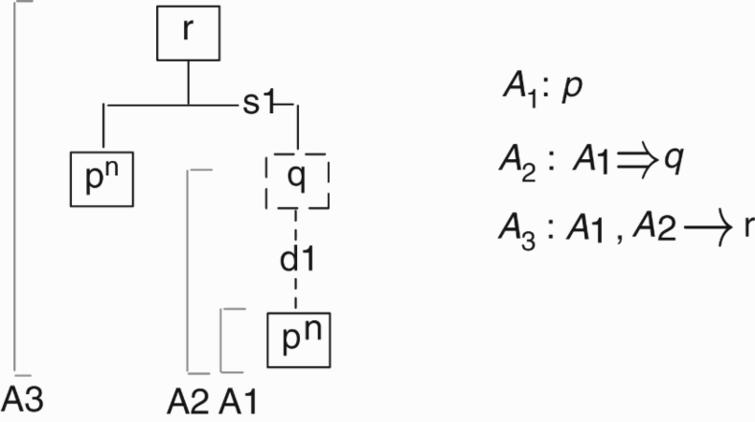
\includegraphics[scale=0.6]{aspic.jpg}
    \caption{Primjer argumenta u ASPIC+ sustavu}
\label{fig:aspic}
\end{figure}

Primjerice, baza podataka se sadrži od:
$p, q, r, s, t, u, v, w, x, d_1, d_2, d_3, d_4, d_5, d_6$ i njihovih negacija, gdje 
je skup strogih pravila $R_s = \{s_1, s_2\}$, a skup oborivih pravila
$R_d = \{d_1, d_2, d_3, d_4, d_5, d_6\}$. Sama pravila su:
\begin{align*}
    d_1&: p \Rightarrow q  &   d_4&: u \Rightarrow v   &    s_1&: p, q \rightarrow r \\
    d_2&: s \Rightarrow t  &   d_5&: v, x \Rightarrow \neg t  &    s_2&: v \rightarrow \neg s \\
    d_3&: t \Rightarrow \neg d_1  &  & d_6 s \Rightarrow \neg p
\end{align*}
Funkcija $n$ pridjeljuje oborivom pravilu $d_i$ formulu $d_i$, dakle vrijedi:
$n(d_i) = d_i$, prikazano na primjeru: $n(p \Rightarrow q) = d_1$. Ovako definiran argument
prikazan je slikom~\ref{fig:aspic}: premise su na dnu slike, a zaključak na vrhu. Premise
su označene eksponentom, a oborive premise i zaključivanja isprekidanom linijom. 
Sada je i upitima moguće doći do elemenata argumenata $A_1, A_2$ i $A_3$. Tako je
$Prem(A_3) = \{p\}$, $DefRules(A_3) = \{d_1\}$. Još primjera i pojašnjenja ASPIC+
radne okoline moguće je pronaći u \citep{modgil2014aspic+}. 

\section{TOAST}

TOAST \engl{The Online Argument Structures Tool} je implementacija ASPIC+ 
\citep{modgil2014aspic+} argumentacijskog okruženja. TOAST je web servis 
u koji je moguće unijeti argumente i evaluirati ih. 
Korisnik TOAST-a može unositi izjave u bazu znanja \engl{knowledge base}
i definirati vlastita pravila \engl{rules} (prema ASPIC+-u). U bazi znanja 
razlikujemo aksiome, premise i pretpostavke. Osim standardnih logičkih
poveznica koje je moguće unositi između tvrdnji u bazi znanja, 
između premisa i pretpostavki moguće je definirati relacije preferencije. 
Pravila se unose u formatu:
\lstset{language=XML}
\begin{lstlisting}[caption={},label={lst:format},language=XML, captionpos=b]
[jedinstvena oznaka] {lista ancedensa}{implikacija}{konsekvens};
\end{lstlisting}
primjerice pravilo s dvije tvrdnje iz kojih logičkom implikacijom slijedi konsekvens:
\lstset{language=XML}
\begin{lstlisting}[caption={},label={lst:format},language=XML, captionpos=b]
[p] {Student Ivo studira na FER-u, FER je u Zagrebu}{->}{Student Ivo studira u Zagrebu};
\end{lstlisting}
Osim relacija klasične logike, moguće je preferirati tvrdnje (PA-čvor) u formatu:
\lstset{language=XML}
\begin{lstlisting}[caption={},label={lst:format},language=XML, captionpos=b]
    [jedinstvena oznaka pravila a] < [jedinstvena oznaka preferiranog pravila b] 
\end{lstlisting}
Primjeri korištenja TOAST-a vidljivi su na slikama~\ref{fig:toast_in} i~\ref{fig:toast}.
TOAST je u potpunosti integriran s AIFdb (više u odjeljku~\ref{sec:aifdb}), stoga je 
moguće argument kreiran u AIFdb-u evaluirati kroz TOAST.\@

\begin{figure}
    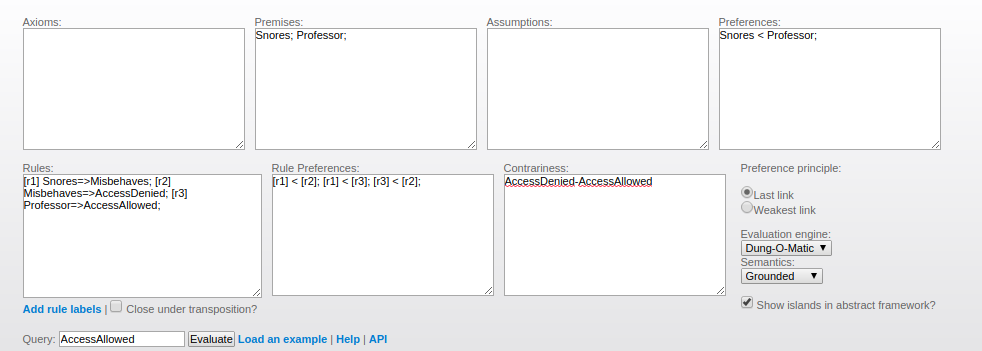
\includegraphics[scale=0.4]{toast_input.png}
    \caption{Unos pravila i baze znanja u TOAST}
\label{fig:toast_in}
\end{figure}

\begin{figure}
    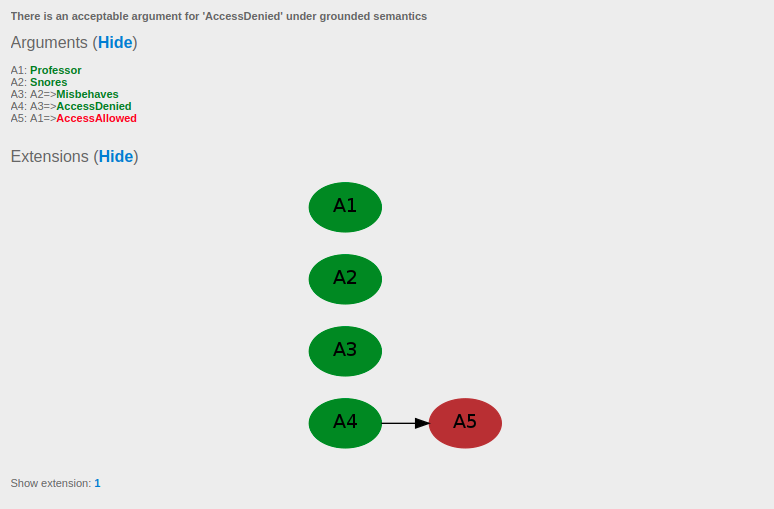
\includegraphics[scale=0.4]{toast.png}
    \caption{Evaluacija prihvatljivosti \emph{AccessDenied} upita}
\label{fig:toast}
\end{figure}
